\documentclass{article}

\def\ParSkip{} 
% Packages
\usepackage{amssymb,amsmath,amsthm,bbm}
\usepackage{verbatim,float,url,dsfont}
\usepackage{graphicx,subfigure,psfrag}
\usepackage{algorithm,algorithmic}
\usepackage{mathtools,enumitem}
\usepackage{multirow}
\usepackage{ragged2e}
\usepackage{xr-hyper}
\usepackage{array}

\usepackage[colorlinks=true,citecolor=blue,urlcolor=blue,linkcolor=blue]{hyperref}
\usepackage[margin=1in]{geometry}
\usepackage[round]{natbib}

\usepackage[utf8]{inputenc} % allow utf-8 input
\usepackage[T1]{fontenc}    % use 8-bit T1 fonts
\usepackage{booktabs}       % professional-quality tables
\usepackage{nicefrac}         % compact symbols for 1/2, etc.
\usepackage{microtype}      % microtypography

\ifdefined\TimesFont 
\usepackage{times} % use times font
\fi

\ifdefined\ParSkip 
\usepackage{parskip} % use par skip
\fi

% Theorems and such
\newtheorem{theorem}{Theorem}
\newtheorem{lemma}{Lemma}
\newtheorem{corollary}{Corollary}
\newtheorem{proposition}{Proposition}
\theoremstyle{definition}
\newtheorem{remark}{Remark}
\newtheorem{definition}{Definition}

% Assumption
\newtheorem*{assumption*}{\assumptionnumber}
\providecommand{\assumptionnumber}{}
\makeatletter
\newenvironment{assumption}[2]{
  \renewcommand{\assumptionnumber}{Assumption #1#2}
  \begin{assumption*}
  \protected@edef\@currentlabel{#1#2}}
{\end{assumption*}}
\makeatother

% Widebar
\makeatletter
\newcommand*\rel@kern[1]{\kern#1\dimexpr\macc@kerna}
\newcommand*\widebar[1]{%
  \begingroup
  \def\mathaccent##1##2{%
    \rel@kern{0.8}%
    \overline{\rel@kern{-0.8}\macc@nucleus\rel@kern{0.2}}%
    \rel@kern{-0.2}%
  }%
  \macc@depth\@ne
  \let\math@bgroup\@empty \let\math@egroup\macc@set@skewchar
  \mathsurround\z@ \frozen@everymath{\mathgroup\macc@group\relax}%
  \macc@set@skewchar\relax
  \let\mathaccentV\macc@nested@a
  \macc@nested@a\relax111{#1}%
  \endgroup
}
\makeatother

% Min and max 
\DeclareMathOperator*{\argmin}{argmin}
\DeclareMathOperator*{\argmax}{argmax}
\DeclareMathOperator*{\minimize}{minimize}
\DeclareMathOperator*{\maximize}{maximize}
\DeclareMathOperator*{\find}{find}
\DeclareMathOperator{\st}{subject\,\,to}

% Other operators
\DeclareMathOperator{\Cov}{Cov}
\DeclareMathOperator{\Var}{Var}
\DeclareMathOperator{\dm}{dim}
\DeclareMathOperator{\col}{col}
\DeclareMathOperator{\row}{row}
\DeclareMathOperator{\nul}{null}
\DeclareMathOperator{\rank}{rank}
\DeclareMathOperator{\nuli}{nullity}
\DeclareMathOperator{\spa}{span}
\DeclareMathOperator{\sign}{sign}
\DeclareMathOperator{\supp}{supp}
\DeclareMathOperator{\diag}{diag}
\DeclareMathOperator{\aff}{aff}
\DeclareMathOperator{\conv}{conv}
\DeclareMathOperator{\dom}{dom}
\DeclareMathOperator{\tr}{tr}
\DeclareMathOperator{\df}{df}

% Other shortcuts 
\def\R{\mathbb{R}}
\def\C{\mathbb{C}}
\def\E{\mathbb{E}}
\def\P{\mathbb{P}}
\def\T{\mathsf{T}}
\def\half{\frac{1}{2}}
\def\df{\mathrm{df}}
\def\hy{\hat{y}}
\def\hf{\hat{f}}
\def\hmu{\hat{\mu}}
\def\halpha{\hat{\alpha}}
\def\hbeta{\hat{\beta}}
\def\htheta{\hat{\theta}}
\def\indep{\perp\!\!\!\perp}
\def\th{^{\textnormal{th}}}

\def\cA{\mathcal{A}}
\def\cB{\mathcal{B}}
\def\cD{\mathcal{D}}
\def\cE{\mathcal{E}}
\def\cF{\mathcal{F}}
\def\cG{\mathcal{G}}
\def\cK{\mathcal{K}}
\def\cH{\mathcal{H}}
\def\cI{\mathcal{I}}
\def\cL{\mathcal{L}}
\def\cM{\mathcal{M}}
\def\cN{\mathcal{N}}
\def\cP{\mathcal{P}}
\def\cS{\mathcal{S}}
\def\cT{\mathcal{T}}
\def\cW{\mathcal{W}}
\def\cX{\mathcal{X}}
\def\cY{\mathcal{Y}}
\def\cZ{\mathcal{Z}}

\usepackage[normalem]{ulem}
\usepackage{centernot}

\title{Lecture 3: Regularization and Smoothing \\ \smallskip  
\large Introduction to Time Series, Fall 2023 \\ \smallskip
Ryan Tibshirani}
\date{}

\begin{document}
\maketitle
\RaggedRight
\vspace{-50pt}

Relevant reading: Chapter 2.3 (smoothing) of Shumway and Stoffer (SS); Chapters
3.3 and 7.7 (smoothing) of Hyndman and Athanasopoulos (HA).

\section{Trouble in high dimensions?} 

\def\new{\text{new}}

\begin{itemize}
\item As in the regression lecture, let's suppose that we seek $\beta \in \R^p$  
  such that for given samples $x_i \in \R^p$ and $y_i \in \R$ (predictor and
  response pairs), $i = 1,\dots,n$,    
  \[
  y_i \approx x_i^\T \beta, \quad  i = 1,\dots,n 
  \]
  (As explained in that lecture, our notation omits the intercept from the
  model, but that is done without a loss of generality, since it can always be
  obtained by appending a coordinate value of 1 to the start of each $x_i$) 

\item Equivalently, we can write $y \in \R^n$ for the response vector (with
  $i\th$ component $y_i$) and $X \in \R^{n \times p}$ for the feature matrix
  (with $i\th$ row $x_i)$, and say that we are seeking $\beta$ such that $y
  \approx X \beta$ 

\item Recall, the least squares estimates of the coefficients are given by
  solving  
  \begin{equation}
  \label{eq:ls}
  \min_{\beta \in \R^p} \, \sum_{i=1}^n (y_i - x_i^\T \beta)^2 \iff
  \min_{\beta \in \R^p} \, \|y - X \beta\|_2^2
  \end{equation}
  where we use $\|\cdot\|_2$ for the Euclidean or $\ell_2$ norm of a vector,
  defined for $a \in \R^d$ as \smash{$\|a\|_2^2 = \sum_{i=1}^d a_i^2$}

\item If $p \leq n$ and $\rank(X) = p$ (here $\rank(X)$ denotes the rank of the 
  matrix $X$), then this produces the unique solution    
  \begin{equation}
  \label{eq:coef}
  \hbeta = (X^\T X)^{-1} X^\T y  
  \end{equation}

\item But if $p > n$, which means we have more features than samples, which we 
  often call the ``high dimensional'' (or ``overparametrized'') setting, then we 
  are in trouble ... the matrix $X^\T X$ cannot be invertible, so the expression
  in \eqref{eq:coef} isn't even well-defined   

\item Moreover, the least squares optimization problem \eqref{eq:ls} does not
  have a unique solution in this case. Indeed, are you'll show on the homework,
  it \smash{$\tilde\beta$} is one solution, then any other vector of the form    
  \begin{equation}
  \label{eq:coef_eta}
  \hbeta = \tilde\beta + \eta, \quad \text{where $\eta \in \nul(X)$}
  \end{equation}
  also solves \eqref{eq:ls}, where $\nul(X)$ is the null space of the matrix
  $X$:
  \[
  \nul(X) = \{ \eta \in \R^p : X \eta = 0 \} 
  \]

\item When $\rank(X) < p$, the null space $\nul(X)$ is nonempty, and since it 
  is a linear space: $\eta \in \nul(X) \implies c \eta \in \nul(X)$ for any $c
  \in \R$, we see that from one least squares solution \smash{$\tilde\beta$}, we
  can generate \emph{infinitely many others} in \eqref{eq:coef_eta} 
  
\item Furthermore, we can always take the ``one least squares solution'' to be:  
  \begin{equation}
  \label{eq:coef_mn}
  \tilde\beta = (X^\T X)^+ X^\T y
  \end{equation}

  \item Here $A^+$ denotes the \emph{generalized inverse} (also called the 
  \emph{Moore-Penrose pseudoinverse}) of a matrix $A$. If you don't know what
  that is, then it doesn't really matter for this lecture, but you can think of
  it precisely as follows: among all solutions in \eqref{eq:ls}, the solution in
  \eqref{eq:coef_mn} is the unique one having the smallest $\ell_2$ norm 
  \smash{$\|\tilde\beta\|_2$} 

\item So, now we come to the discussion of specific \emph{troubles}. There are
  actually two distinct troubles. The first trouble involves the interpretation
  of the coefficients themselves. If we are interested in such interpretations,
  then the $p = n$ barrier is the end of the road for least squares. Why? Once
  $p > n$, and we find any least squares solution \smash{$\tilde\beta$} with
  \smash{$\tilde\beta_j > 0$} for some $j$, then we can always
  find\footnote{Technically, this is only true if $\nul(X) \not \perp e_j$,
    where $e_j$ is the $j\th$ standard basis vector.}  
  another solution \smash{$\hbeta$} of the form \eqref{eq:coef_eta} with
  \smash{$\hbeta_j < 0$}. You will prove this on the homework. Thus we cannot
  even consistently interpret the sign of any of any estimated coefficient (let
  alone its magnitude) 

\item The second trouble involves prediction. The $p = n$ barrier is generally
  disastrous for least squares prediction. If $p < n$ and \smash{$\hat{y}_{\new}
    = x_{\new}^\T \hbeta$} is the least squares prediction at a new predictor
  value \smash{$x_{\new}$} (for \smash{$\hbeta$} the usual least squares
  coefficients in \eqref{eq:coef}), whose associated response is
  \smash{$y_{\new}$}, then under fairly standard conditions for regression
  theory,
% \footnote{This assumes that the true model is linear and the errors are
%   independent of the features (as well as assuming that the data are all
%   i.i.d., and some other mild-ish conditions on the distributions of the
%   errors and features that are not worth mentioning). In other words, it is a
%   fairly idealized model. So the fact that least squares performs poorly here
%   as $p$ approaches $n$, in this model, is especially notable.} 
  the prediction MSE behaves as: 
  \[
  \E \big[ (y_{\new} - \hat{y}_{\new})^2 \big] \approx \sigma^2
  \frac{p}{n-p} 
  \]
  for large $n$ and $p$, where $\sigma^2$ is the error variance. What do we
  notice? This explodes as $p$ approaches $n$. Big problem!

\item (Aside: what happens with the prediction MSE when $p > n$? The answer may
  surprise you. The MSE associated with the particular solution in
  \eqref{eq:coef_mn} is actually quite interesting and in some ways exotic when 
  $p > n$. Typically we need $p$ to be \emph{much larger} than $n$ (away from
  the $p = n$ barrier) in order for it to be well-behaved. This has been the
  topic of a recent flurry of research in statistics in machine learning ...  we
  won't focus on it in this lecture and will instead talk about explicit
  regularization. But feel free to ask about it in office hours)    
\end{itemize}

\section{Regularization}

\begin{itemize}
\item \emph{Regularization} to the rescue! This will finesse both of the
  problems described above: it gives us a way to produce nontrivial coefficient 
  estimates, and it often gives us more accurate predictions 

\item In the regression setting, a general approach for regularization moves us 
  from \eqref{eq:ls} to solving:
  \begin{equation}
  \label{eq:ls_pen}
  \min_\beta \; \|y - X\beta\|_2^2 + \lambda P(\beta)
  \end{equation}
  Here $P : \R^p \to \R_+$ is some penalty function, and $\lambda \geq 0$ is a
  tuning parameter (also called the regularization parameter) which trades off
  the importance of the squared loss---first term in \eqref{eq:ls_pen}, and the
  penalty---second term in \eqref{eq:ls_pen}  

\item In other words, the larger the value of $\lambda$, the more weight we put
  on penalizing large values of $P(\beta)$, which results in estimates that we
  call more ``regularized''   

\item Arguably the three canonical choices for penalties are based on the
  $\ell_0$, $\ell_1$, and $\ell_2$ norms:   
  \begin{align*}
  P(\beta) &= \|\beta\|_0 = \sum_{j=1}^p 1\{\beta_j \not= 0\}, \\
  P(\beta) &= \|\beta\|_1 = \sum_{j=1}^p |\beta_j|, \\
  P(\beta) &= \|\beta\|_2^2 = \sum_{j=1}^p \beta_j^2.
  \end{align*}
  This gives rise to what we call \emph{best subset selection}, the
  \emph{lasso}, and \emph{ridge regression}, respectively

\item (Aside: calling $\|\cdot\|_0$ the ``$\ell_0$ norm'' is a misnomer, as it
  is not actually a norm: it does not satisfy positive homogeneity, i.e.,
  $\|a\beta\|_0 = a\|\beta\|_0$ for all $a>0$. It would be more accurate to
  call it the ``$\ell_0$ pseudonorm'', but nearly everybody just calls it the
  ``$\ell_0$ norm'')

\item Critically, $\|\cdot\|_0$ is \emph{not convex}, while $\|\cdot\|_1$ and 
  $\|\cdot\|_2$ are convex (note that any norm is a convex function). This makes
  best subset selection a nonconvex problem, and one that is generally very hard
  to solve in practice except for small $p$. We won't focus on best subset 
  selection further in this lecture. (Though it is itself the topic of a flurry 
  of work in the operations research literature a few years ago ... which you
  can ask about in office hours if you are curious) 

\item Lastly, an important note: when there is an explicit intercept $\beta_0$
  in the model, we typically do not want to penalize it, \emph{and so we modify
    the penalty $P(\beta)$ so that it excludes $\beta_0$}---this will be
  implicit in everything below 

\item Ok, really lastly, penalties like $\ell_1$ and $\ell_2$ only make sense if
  all the features (columns of $X$) are on the same scale (why?). Thus an 
  important and standard preprocessing step is to scale each feature (column of
  $X$) so that it has unit sample variance 
\end{itemize}

\subsection{Ridge}

\begin{itemize}
\item The \emph{ridge} estimates of regression coefficients are given by solving    
  \[
  \min_{\beta \in \R^p} \, \sum_{i=1}^n (y_i - x_i^\T \beta)^2 + \lambda
  \sum_{j=1}^p \beta_j^2
  \]
  or equivalently
  \begin{equation}
  \label{eq:ridge}
  \min_{\beta \in \R^p} \, \|y - X \beta\|_2^2 + \lambda \|\beta\|_2^2
  \end{equation}

\item The problem in \eqref{eq:ridge} has closed-form solution, verified by  
  differentiating the criterion and setting the result equal to zero,
  \begin{equation}
  \label{eq:coef_ridge}
  \hbeta = (X^\T X + \lambda I)^{-1} X^\T y
  \end{equation}
  where $I$ is in the $p \times p$ identity matrix. This \emph{always exists}
  (the matrix $X^\T X + \lambda I$ is always invertible), regardless of the
  relative sizes of $n,p$

\item Figure \ref{fig:cardio} gives an example of the ridge regression
  coefficient estimates as a function of $\lambda$, fit on the cardiovascular 
  mortality regression data, with many features derived from lags of particulate 
  levels 

\begin{figure}[p]
\centering
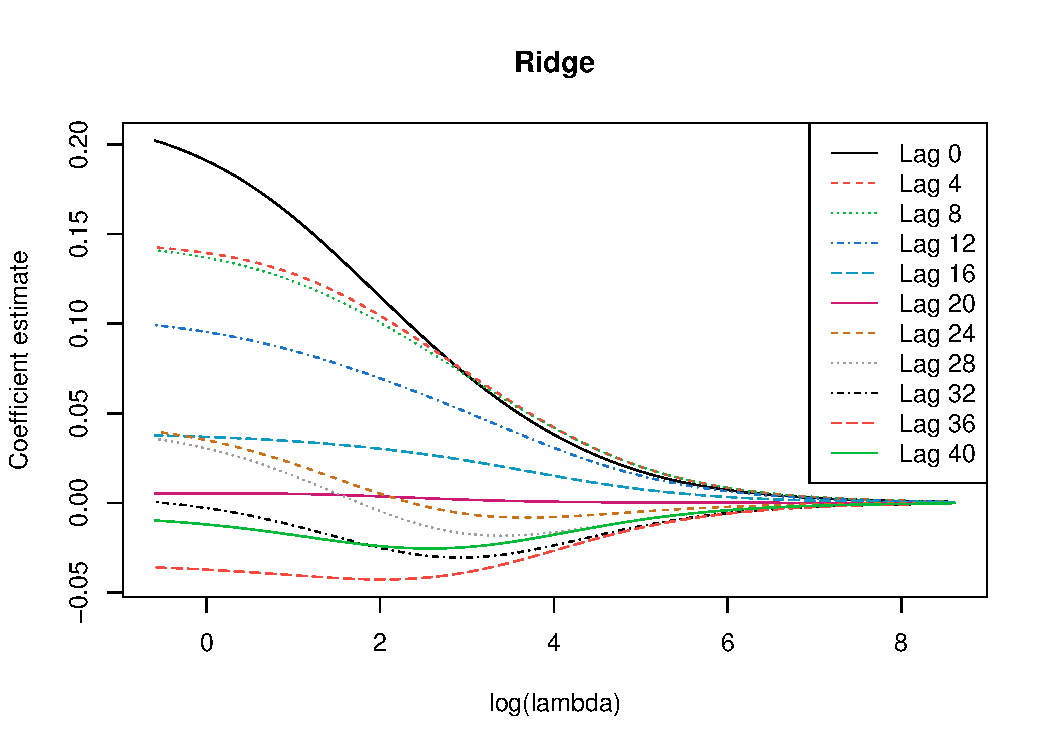
\includegraphics[width=0.875\textwidth]{fig/cardio-ridge-1.pdf}
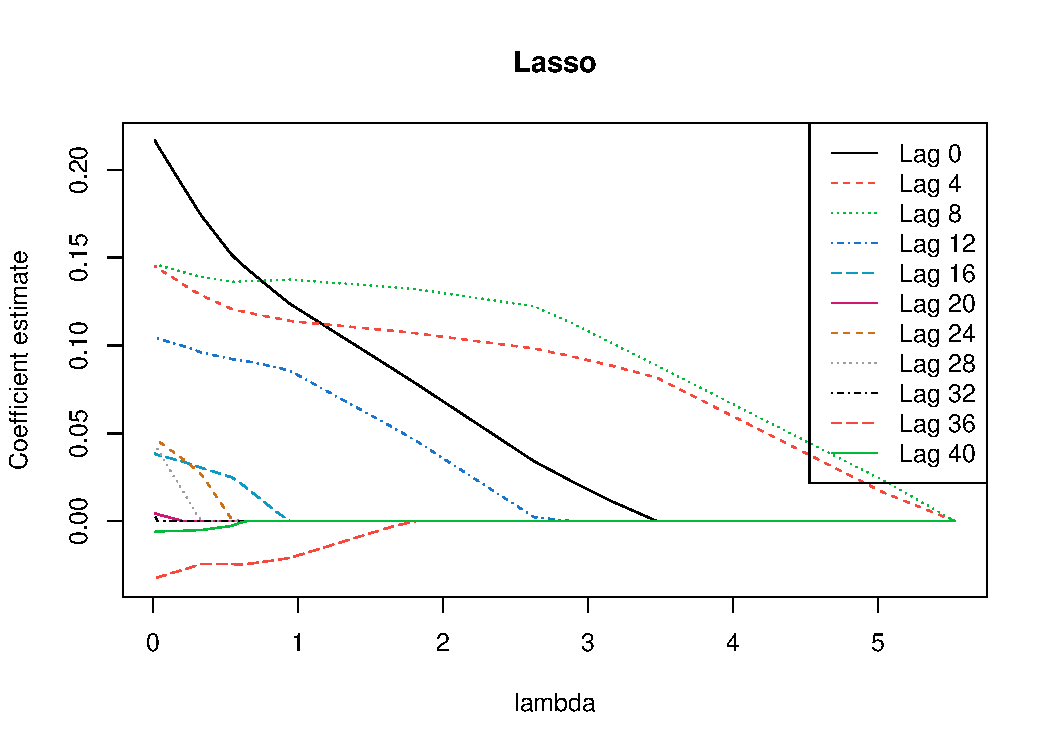
\includegraphics[width=0.875\textwidth]{fig/cardio-lasso-1.pdf}
\caption{Ridge and lasso estimates on the cardiovascular mortality regression
  problem, with lags of particulate levels as features. (The intercept is
  estimated without a penalty, and omitted from the plots for visualization 
  purposes)} 
\label{fig:cardio}
\end{figure}
\end{itemize}

\subsection{Lasso}

\begin{itemize}
\item The \emph{lasso} estimates of regression coefficients are given by solving    
  \[
  \min_{\beta \in \R^p} \, \sum_{i=1}^n (y_i - x_i^\T \beta)^2 + \lambda
  \sum_{j=1}^p |\beta_j|
  \]
  or equivalently
  \begin{equation}
  \label{eq:lasso}
  \min_{\beta \in \R^p} \, \|y - X \beta\|_2^2 + \lambda \|\beta\|_1
  \end{equation}

\item There are a number of key differences between the ridge \eqref{eq:ridge}
  and \eqref{eq:lasso} problems (and estimator). First, the lasso problem does
  not have a closed-form solution (it does not even necessarily always admit a
  unique solution; though it is essentially always unique if we have
  continuously distributed features)

\item A second key difference is that the lasso estimates of the regression
  coefficients are \emph{sparse}. In other words, solving the lasso problem
  results in a vector \smash{$\hbeta$} with many components exactly equal to
  zero, and a larger choice of $\lambda$ will result in more zeros. This doesn't
  happen with ridge regression, whose coefficient estimates are generically
  \emph{dense}. Figure \ref{fig:lasso_ridge} is the ``classic'' picture used to
  explain this, and we will talk through its interpretation in lecture 

\begin{figure}[htb]
\centering
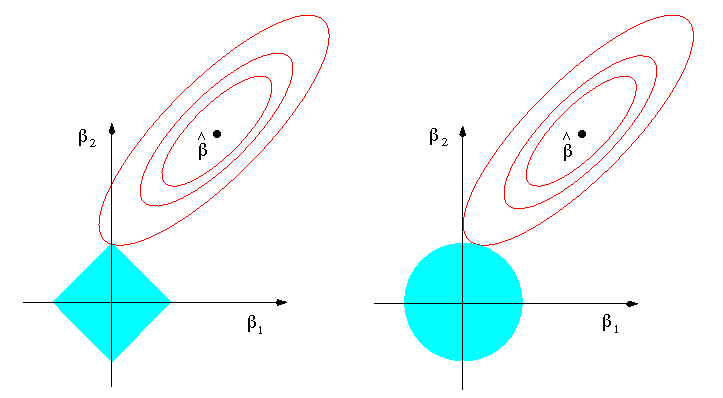
\includegraphics[width=0.95\textwidth]{lasso_ridge.pdf}
\caption{\it The ``classic'' illustration comparing lasso and ridge, each in
  constrained form (from ``Elements of Statistical Learning'' by Hastie,
  Tibshirani, and Friedman)}
\label{fig:lasso_ridge}
\end{figure}

\item See Figure \ref{fig:cardio} again for an example of the lasso coefficients
  on the cardiovascular mortality data. We can see that as $\lambda$ grows, it
  sets many of the coefficients of lagged features to zero

\item In general, this sparsity-inducing behavior of the $\ell_1$ penalty allows
  the lasso to perform \emph{variable selection} in the working linear model. By
  zero-ing out some coefficients exactly, it discards some features from having
  any predictive influence in the fitted model. Which precise features it
  discards is chosen based on the data. Many people like sparsity because it
  leads to better interpretability  
\end{itemize}

\subsection{Discussion}

\begin{itemize}
\item We should be clear that the lasso is not ``better'' than ridge, in any
  general sense, and neither is ridge ``better'' than the lasso. They each can
  help tremendously with stabilizing coefficient estimates so as to lead to
  improved predictive accuracy. They each do so by regularizing in different
  ways 

\item The most basic question to ask: is a sparse linear model likely
  to be a good (or desirable) approximation to the true regression function? If
  so, then the lasso can outperform (or be preferable) to ridge. On the other 
  hand, in problems where there are many underlying features that are relevant
  for prediction, ridge can outperform the lasso 

\item (And often times people combine the two penalties which gives rise to the
  \emph{elastic net}) 

\item There is a lot more to say---in terms of connections to other ideas in
  statistics, extensions, and so on---but we won't be able to cover it in this
  class. We'll simply view ridge and lasso as tools that allow us to consider 
  many more features than we would otherwise feel comfortable including in
  traditional regression models, and then regularize in order to control
  variance (stabilize estimates)   

\item In time series regression, in the vein of examples we studied in the last 
  lecture, this would allow us to include \emph{many lags} of a feature of
  interest, or a few lags of \emph{many external covariates}, and so on, and
  then apply a ridge or lasso penalty. Then, you might wonder: how would we
  select $\lambda$? In fact, you already know the answer (for problems with a
  predictive focus): use time series cross-validation!

\item That is, define a grid of $\lambda$ values, fit ridge or lasso estimates
  for each $\lambda$, let each one make predictions, and select the value that 
  yields the best CV error. You will practice this on the homework, where you'll
  also use the \verb|glmnet| package to solve the ridge and lasso problems 
\end{itemize}

\section{Smoothing}

\begin{itemize}
\item Shifting gears, we'll now talk about \emph{smoothing}, which for us will
  be a task that is mainly about retrospective rather than prospective
  estimation (as in forecasting)

\item As with regression, most smoothing techniques are not actually specific to
  time series data, so our notation will be generic to reflect this. There are
  so many smoothers out there, and we will choose three ones to discuss that are
  generic in principle, but are quite popular (and in part, have roots in) the
  time series context  

\item Recall the signal plus noise model from our earlier lectures, 
  \[
  y_i =\theta_i + \epsilon_i, \quad i = 1,\dots,n
  \]
  where $\epsilon_i$, $i=1,\dots,n$ are white noise errors, and $\theta_i$, $i =
  1,\dots,n$ denote the unknown means that we want to estimate, assumed to be
  smoothly varying across the index $i$

\item Two broad classes of smoothers of interest are as follow. The first are
  \emph{linear filters}, which are (weighted) local averages, of the form  
  \begin{equation}
  \label{eq:smooth_lin}
  \htheta_i = \sum_{j=-k}^k a_j y_{i-j},\quad i = 1,\dots,n
  \end{equation}
  for some weights $a_j$, $j = 1,\dots,m$

\item The second are \emph{penalized least squares} smoothers, which are given
  by solving    
  \begin{equation}
  \label{eq:smooth_pen}
  \min_{\theta \in \R^n} \, \sum_{i=1}^n (y_i - \theta_i)^2 + \lambda P(\theta) 
  \end{equation}
  for some penalty function $P : \R^n \to \R_+$ and tuning parameter $\lambda 
  \geq 0$   

\item You should be able to clearly see the connection between smoothing and
  regularization, with \eqref{eq:smooth_pen} being a special case of
  \eqref{eq:ls_pen} (when $X = I$, the identity matrix). Note, the choice of
  penalties that are common and useful in smoothing, as we'll see below, are
  more complex than simple $\ell_1$ or $\ell_2$ penalties  

\item There is a broader connection between smoothing and regression, embodied
  by what is called an \emph{additive model}. In one sentence: this is a
  regression, but with individual features replaced by nonlinear transforms of
  features, where the nonlinearities are fit by smoothers. We'll very briefly
  return to this at the end
\end{itemize}

\subsection{Linear filters}

\begin{itemize}
\item A \emph{moving average} (MA), either of centered or trailing type, is one
  of the basic and widely-used examples of a linear filter, of the form 
  \eqref{eq:smooth_lin}. For a window of (odd) length $m = 2k+1$, a centered MA
  smoother uses weights 
  \[
  a_{-k} = \cdots a_0 = \cdots = a_k = \frac{1}{m}
  \]
  For a window of (odd or even) length $m = k+1$, a trailing MA smoother uses
  weights 
  \[
  a_{-k} \cdots a_0 = \frac{1}{m}
  \]

\item (For either, centered or trailing MA smoothers, or really linear filters
  in general, there will be annoying boundary issues to pay attention to
  ... some software packages may just pad the response vector with 0s in order
  to deal with them; but a more principled approach is probably to renormalize
  the weights at the boundaries so that the filter is averaging over the
  ``right'' number of observations; and the safest approach is to just omit 
  estimates at the boundaries, i.e., report NAs)

\item Figure \ref{fig:soi} displays an example of centered MA smoothing on the 
  Southern Oscillation Index (SOI), which measures air pressure in the Central 
  Pacific Ocean. We can see that the results look fairly accurate (they track
  the known cycles which occur every 3-7 years, due to the El Nino effect), but
  the estimates look a bit ``choppy''    

\begin{figure}[p]
\centering
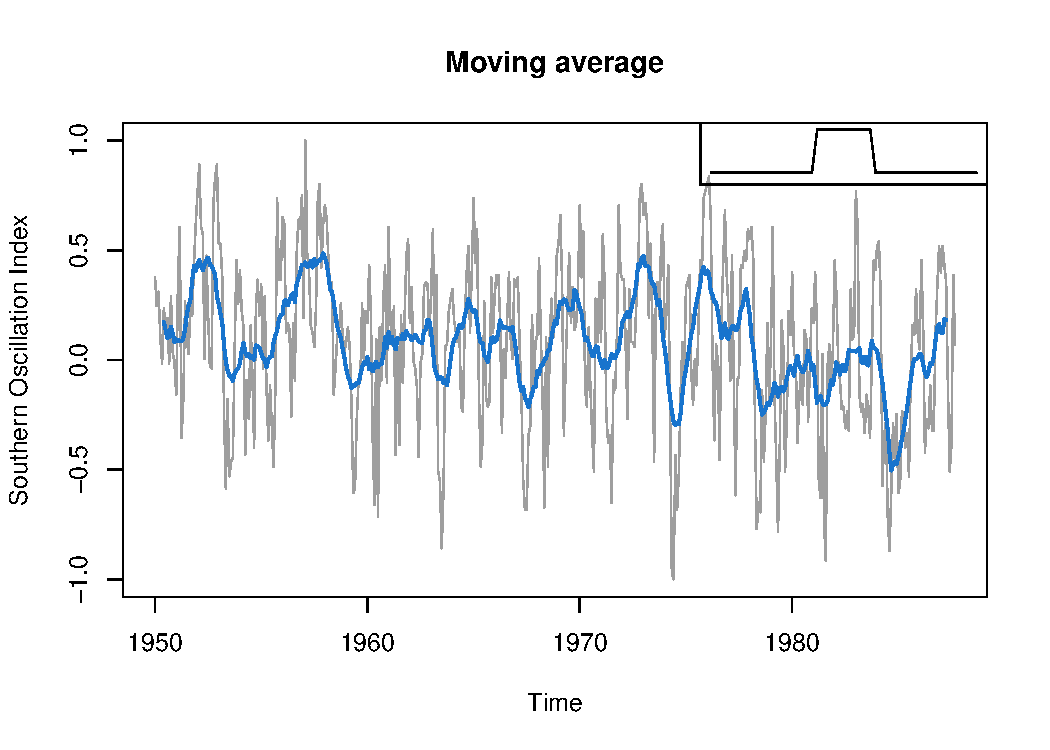
\includegraphics[width=0.875\textwidth]{fig/soi-ma-1.pdf}
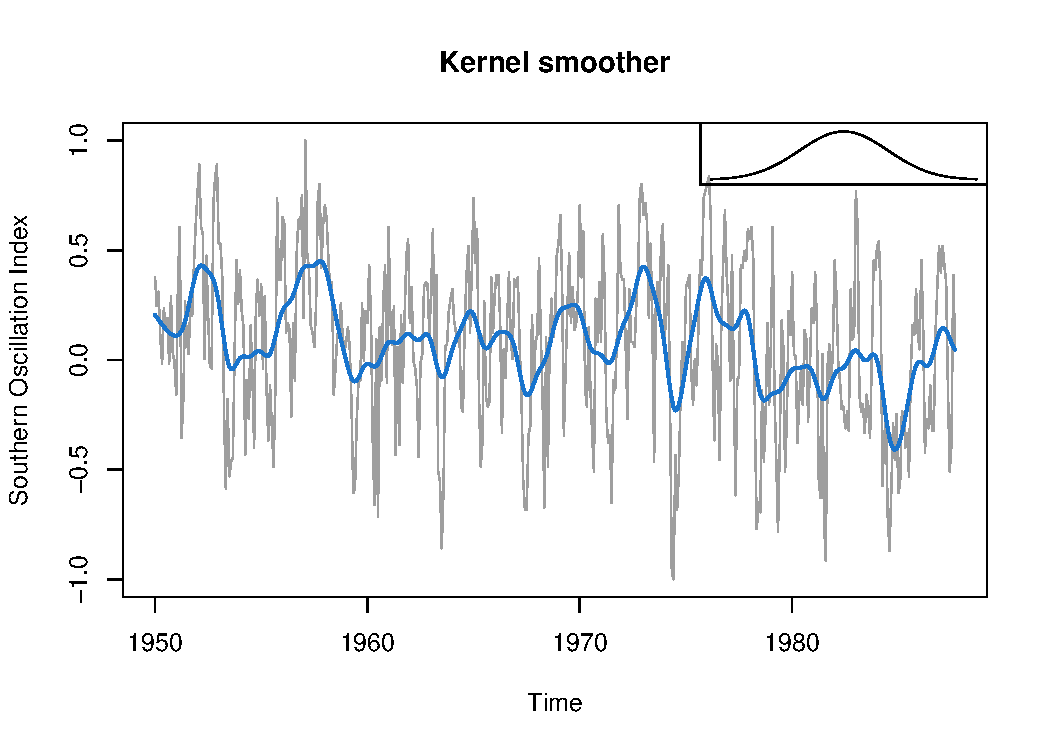
\includegraphics[width=0.875\textwidth]{fig/soi-ks-1.pdf}
\caption{Moving average and Gaussian kernel smoothing estimates fit to the
  Southern Oscillation Index (from SS).}  
\label{fig:soi}
\end{figure}

\item We can get smoother-looking estimates by using a smoother weight sequence
  (with larger $k$). This is precisely what \emph{kernel smoothing} does: it
  uses $k = n$ and 
  \[
  a_j = \frac{K(j/b)}{\sum_{i=1}^n K(i/b)}, \quad j = 1,\dots,n 
  \]
  for a particular \emph{kernel function} $K : \R \to \R$ and \emph{bandwidth}
  $b$. Think of the bandwidth as a tuning parameter, just like the
  regularization level $\lambda$ in ridge or lasso 

\item A common choice of kernel is the Gaussian kernel, $K(u) =
  e^{-u^2/2}$. Figure \ref{fig:soi} gives an example of Gaussian kernel
  smoothing on the SOI data again. We can see that the estimates look more
  smooth  

\item (Note that a centered MA is a special case of kernel smoothing with a
  ``boxcar'' kernel: $K(u) = 1\{|u| \leq b\}$)
\end{itemize}

\subsection{Hodrick-Prescott filter}

\begin{itemize}
\item The \emph{Hodrick-Prescott filter}, or simply HP filter, is a penalized 
  estimator of the form \eqref{eq:smooth_pen}, defined by 
  \begin{equation}
  \label{eq:hp_filter}
  \min_{\theta \in \R^n} \, \sum_{i=1}^n (y_i - \theta_i)^2 + \lambda
  \sum_{i=1}^{n-2} (\theta_i - 2\theta_{i+1} + \theta_{i+2})^2
  \end{equation}

\item We can see that the penalty is squared $\ell_2$ norm of the terms
  $\theta_i -  2\theta_{i+1} + \theta_{i+2}$, $i = 1,\dots,n-2$. Each of these
  are a \emph{second difference} of $\theta$, centered at a particular index 

\item The HP filter is named after two econometricians who proposed the idea in
  the early 1980s. But it is worth noting that very similar ideas were around
  much, much early (the idea of penalizing according to squared first
  differences dates back to the 1899, and according to squared third differences
  dates back to 1923)    

\item Like the ridge problem, which is similar in spirit (but aimed at solving a 
  different problem), the HP filter problem \eqref{eq:hp_filter} has an exact 
  solution. First define the second difference matrix $D \in \R^{(n-2) \times
    n}$ by 
  \begin{equation}
  \label{eq:d_mat}
  D = \begin{bmatrix}
  1 & -2 & 1 & 0 & 0 & \cdots & 0 & 0 & 0 \\
  0 & 1 & -2 & 1 & 0 & \cdots & 0 & 0 & 0 \\
  0 & 0 & 1 & -2 & 1 & \cdots & 0 & 0 & 0 \\
  \vdots & & & \cdot & & & \\
  0 & 0 & 0 & 0 & 0 & \cdots & 1 & -2 & 1 \\
  \end{bmatrix}
  \end{equation}
  and then rewrite the HP filter optimization problem \eqref{eq:hp_filter} as 
  \begin{equation}
  \label{eq:hp_filter2}
  \min_{\theta \in \R^n} \, \|y - \theta\|_2^2 + \lambda \|D \theta\|_2^2 
  \end{equation}

\item The HP filter solution can be derived by differentiating the criterion in
  \eqref{eq:hp_filter2}, setting it equal to zero, and solving, which yields 
  \begin{equation}
  \label{eq:theta_hp}
  \htheta = (I + \lambda D^\T D)^{-1} y
  \end{equation}

\item Figure \ref{fig:boston} shows an example of the HP filter fit to the
  winning men's times from the Boston marathon, at a few different values of the
  regularization level $\lambda$

\item The HP filter has a computational advantage a linear filter with smooth
  weights, such as the Gaussian kernel smoother (the HP filter can be computed
  in linear-time because $D$ is banded). In terms of the qualitative behavior of
  their estimates, the HP filter and Gaussian kernel smoother are pretty similar    

\item In fact, though it not obvious at all, the HP filter admits an
  \emph{equivalent} form as a kernel smoother, for a special implicit kernel 
  (you will study this as a bonus problem on the homework) 

\item The HP filter is worth knowing about because it is quite a popular tool in
  macroeconomics, where it is primarily used for time series decomposition: it
  is used to estimate a trend component in a time series, and then the residuals
  from this are used to estimate a cyclic component. However, some
  econometricians have recently criticized this practice, on the basis that it
  can induce spurious correlations in the residuals, along with other
  concerns.\footnote{See Hamilton ``Why you should never use the
    Hodrick-Prescott filter'' (2017), but also Hodrick ``An exploration of
    trend-cycle decomposition methodologies in simulated data'' (2020), which is
    a rebuttal that challenges some of the ideas proposed by Hamilton. Hodrick
    finds empirically that the HP filter does a better job of isolating the
    cyclic component (in simulation) than the regression method proposed by 
    Hamilton.}  

\item Another reason worth learning about the HP filter is that it provides us a
  natural bridge to another method that we'll cover next, which acts completely 
  differently from any linear filter
\end{itemize}

\subsection{Trend filter}

\begin{itemize}
\item The \emph{$\ell_1$ trend filter}, or simply trend filter, is another
  penalized estimator of the form \eqref{eq:smooth_pen}, defined by     
  \begin{equation}
  \label{eq:trend_filter} 
  \min_{\theta \in \R^n} \, \sum_{i=1}^n (y_i - \theta_i)^2 + \lambda
  \sum_{i=1}^{n-2} |\theta_i - 2\theta_{i+1} + \theta_{i+2}|
  \end{equation}

\item We can see that the penalty is the $\ell_1$ norm of second differences of
  $\theta$. Thus, compared do the HP filter, the only difference is in the use
  of an $\ell_1$ norm penalty, and not squared $\ell_2$ norm penalty

\item Just as in \eqref{eq:hp_filter2}, we can rewrite the trend filter
  \eqref{eq:trend_filter} more compactly as
  \begin{equation}
  \label{eq:trend_filter2}
  \min_{\theta \in \R^n} \, \|y - \theta\|_2^2 + \lambda \|D \theta\|_1 
  \end{equation}
  where $D \in \R^{(n-2) \times n}$ is the second difference matrix in
  \eqref{eq:d_mat} 

\item Swapping the squared $\ell_2$ penalty with an $\ell_1$ penalty on second
  differences results in a \emph{very} different behavior in the estimator. 
  Think of the analogy of ridge versus the lasso. Trend filtering yields
  estimates that are \emph{sparse} in second differences: if we denote by
  \smash{$\htheta$} the solution vector in \eqref{eq:trend_filter2}, then many
  components of \smash{$D \htheta$} will be exactly equal to zero, and a larger
  choice of $\lambda$ will generally result in more zeros 

\item Since 
  \[
  \htheta_i - 2\htheta_{i+1} + \htheta_{i+2} = 0 \iff  
  \htheta_{i+1} = \frac{\htheta_i + \htheta_{i+2}}{2} 
  \]
  this means that many components \smash{$\htheta_i$} will lie on the line
  defined by their neighbors

\item Or in other words, the trend filter solution \smash{$\htheta$} will have a
  \emph{piecewise linear} structure, with a kink at each point $i$ such that
  \smash{$\htheta_{i+1} \not= (\htheta_i + \htheta_{i+2})/2$}. These kink points
  (also called knot points) are chosen adaptively, based on the data

\begin{figure}[p]
\centering
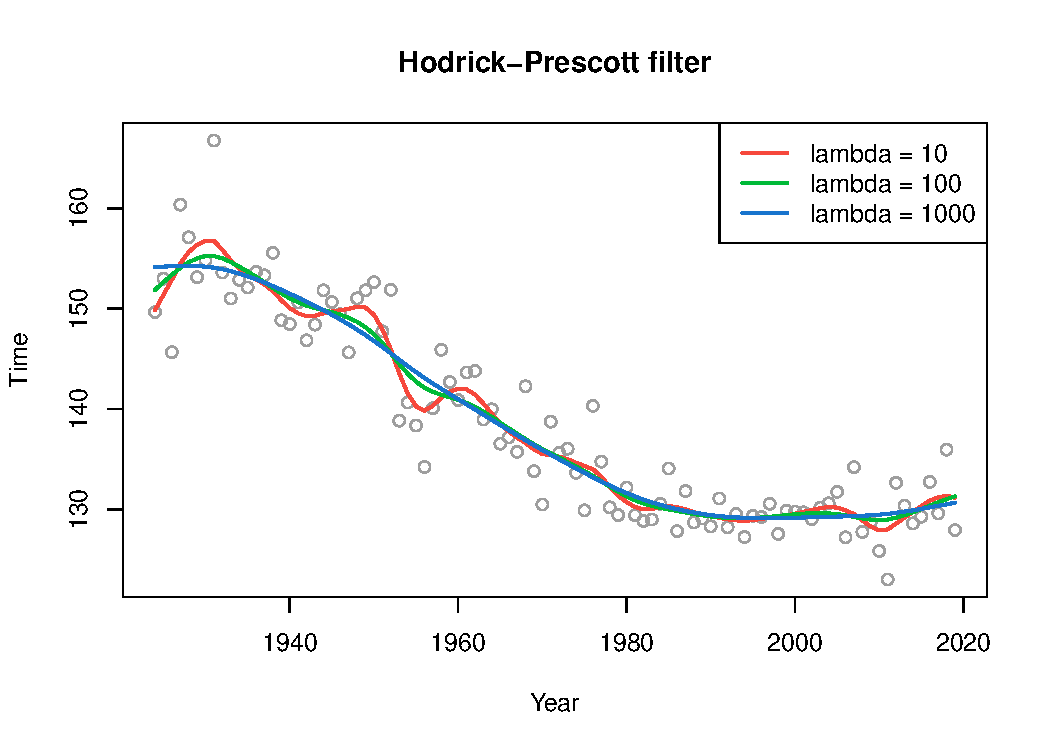
\includegraphics[width=0.875\textwidth]{fig/boston-hp-1.pdf}
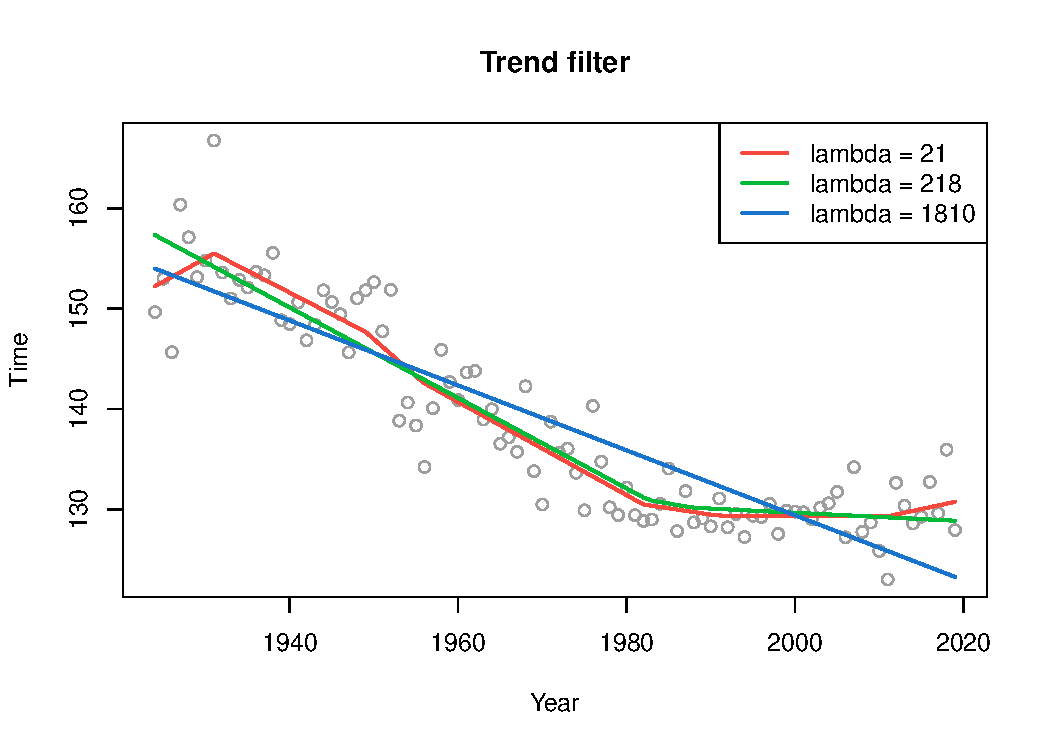
\includegraphics[width=0.875\textwidth]{fig/boston-tf-1.pdf}
\caption{HP filter and trend filter estimates fit to the winning men's Boston
  marathon times (from HA), each at a few different values of $\lambda$.}    
\label{fig:boston}
\end{figure}

\item Figure \ref{fig:boston} shows an example of the trend filter on Boston
  marathon data again. The piecewise linear structure, and qualitative
  difference to the HP filter, is very clear. (Ask yourself: what estimate does
  trend filtering return as $\lambda \to \infty$?) 

\item So ... how do you choose the regularization level $\lambda$ in the trend 
  filter or HP filter, or bandwidth $b$ in a kernel smoother? Cross-validation!
  (Are you tired of that answer by now?) This is actually closer to traditional
  CV, rather than time series CV (since we are not in a forecasting setting,
  where we are predicting the future), but just more structured in how we form
  the folds

\item To tune any one of the smoothers described above, we can define (say) 5
  folds using every $5\th$ point in the sequence. That is, we leave out every
  $5\th$ point, fit the smoother on the remaining points, over a grid of tuning 
  parameter values, and calculate the squared error on the held-out
  points.\footnote{To form an estimate at each held-out point, we can use
    linear interpolation of the estimates at its neighbors.} 
  Doing this 4 more times, where each time we shift the indices of the held-out
  points forward by one, we will be able to compute the average error over all
  points, and use this to select the tuning parameter value. You'll implement
  this on the homework  
\end{itemize}

\section{Additive models}

\begin{itemize}
\item To gear up to (very) briefly discuss additive models, we have to first
  make clear the following point: \emph{each one of the smoothers described in
    the last section can be extended to a problem where the input points in the
    underlying smoothing problem are arbitrary: $x_i$, $i = 1,\dots,n$ (rather
    than simply $x_i = i$, as would be the case in standard time series)}

\item Now let's introduce the \emph{additive model}. This extends the basic
  multivariate linear regression model:
  \[
  y_i \approx \beta_0 + \sum_{j=1}^p \beta_j x_{ij}, \quad i = 1,\dots,n
  \]
  to 
  \[
  y_i \approx \beta_0 + \sum_{j=1}^p f_j(x_{ij}), \quad i = 1,\dots,n
  \]
  where each $f_j$ is a smooth transformation to be estimated

\item In other words, we have moved from estimating linear transformations of
  the features to \emph{nonlinear} ones, which we fit using a smoother
  (traditional packages use kernel smoothing, or spline smoothing, which is
  similar to using the HP filter) 

\item This can be super useful, and hopefully you'll learn about this in more
  detail in your regression class (or some advanced modeling class). For us, it
  is only an idea mentioned in passing, but you'll get to work with an additive
  model on the homework 
\end{itemize}
\end{document}
